\documentclass{article}
\usepackage{listings}
\usepackage{mathrsfs}
\usepackage[utf8]{inputenc}
\usepackage{amssymb}
\usepackage{lipsum}
\usepackage{amsmath}
\usepackage{fancyhdr}
\usepackage{geometry}
\usepackage{scrextend}
\usepackage[english,german]{babel}
\usepackage{titling}
\setlength{\droptitle}{-3cm}
\usepackage{tikz}
\usepackage{algorithm,algpseudocode}
\usepackage[doublespacing]{setspace}
\usetikzlibrary{datavisualization}
\usetikzlibrary{datavisualization.formats.functions}
\usepackage{polynom}
\usepackage{amsmath}
\usepackage{gauss}
\usepackage{tkz-euclide}
\usetikzlibrary{datavisualization}
\usetikzlibrary{datavisualization.formats.functions}
\author{
Alexander Mattick Kennung: qi69dube\\
Kapitel 1
}
\usepackage{import}
\date{\today}
\geometry{a4paper, margin=2cm}
\usepackage{stackengine}
\parskip 1em
\newcommand\stackequal[2]{%
  \mathrel{\stackunder[2pt]{\stackon[4pt]{=}{$\scriptscriptstyle#1$}}{%
  $\scriptscriptstyle#2$}}
 }
\makeatletter
\renewcommand*\env@matrix[1][*\c@MaxMatrixCols c]{%
  \hskip -\arraycolsep
  \let\@ifnextchar\new@ifnextchar
  \array{#1}}
\makeatother
\lstset{
  language=haskell,
}
\lstnewenvironment{code}{\lstset{language=Haskell,basicstyle=\small}}{}
\usepackage{enumitem}
\setlist{nosep}
\usepackage{titlesec}

\titlespacing*{\subsection}{0pt}{2pt}{3pt}
\titlespacing*{\section}{0pt}{0pt}{5pt}
\titlespacing*{\subsubsection}{0pt}{1pt}{2pt}
\title{Vorlesung 4}


\begin{document}
	\maketitle
	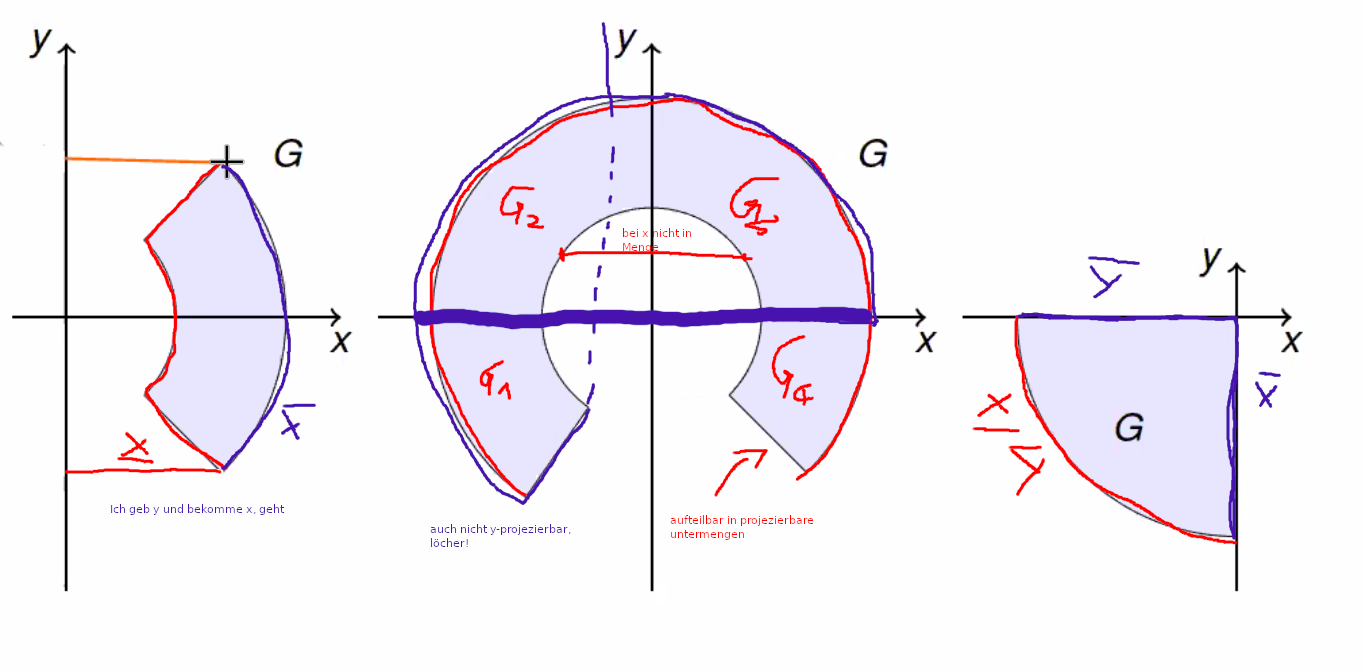
\includegraphics[width=256px]{projezierbarkeit.png}\\
	Urnenmodell $P(A)=\frac{|A|}{|\Omega|}$\\
	alternativ allerdings:\\
	1. Stufe 1 aus 40 Kugeln $P(A_1)=\frac{|A_1|}{|\Omega_1|}$ (also alle guten optionen der optionen, die man im schritt 1 hat)\\
	2. Stufe 1 aus 39 \dots\\
	z.B.: $A_{3394}$\\
	1. Stufe $A_1= 1 von 4 vierern: P(A_1)=\frac{4}{40}$\\
	2. Stufe $A_2= 1 von 3 vierern: P(A_2)=\frac{3}{39}$\\
	3.Stufe $4/38$\\
	4. Stufe $4/37$\\
	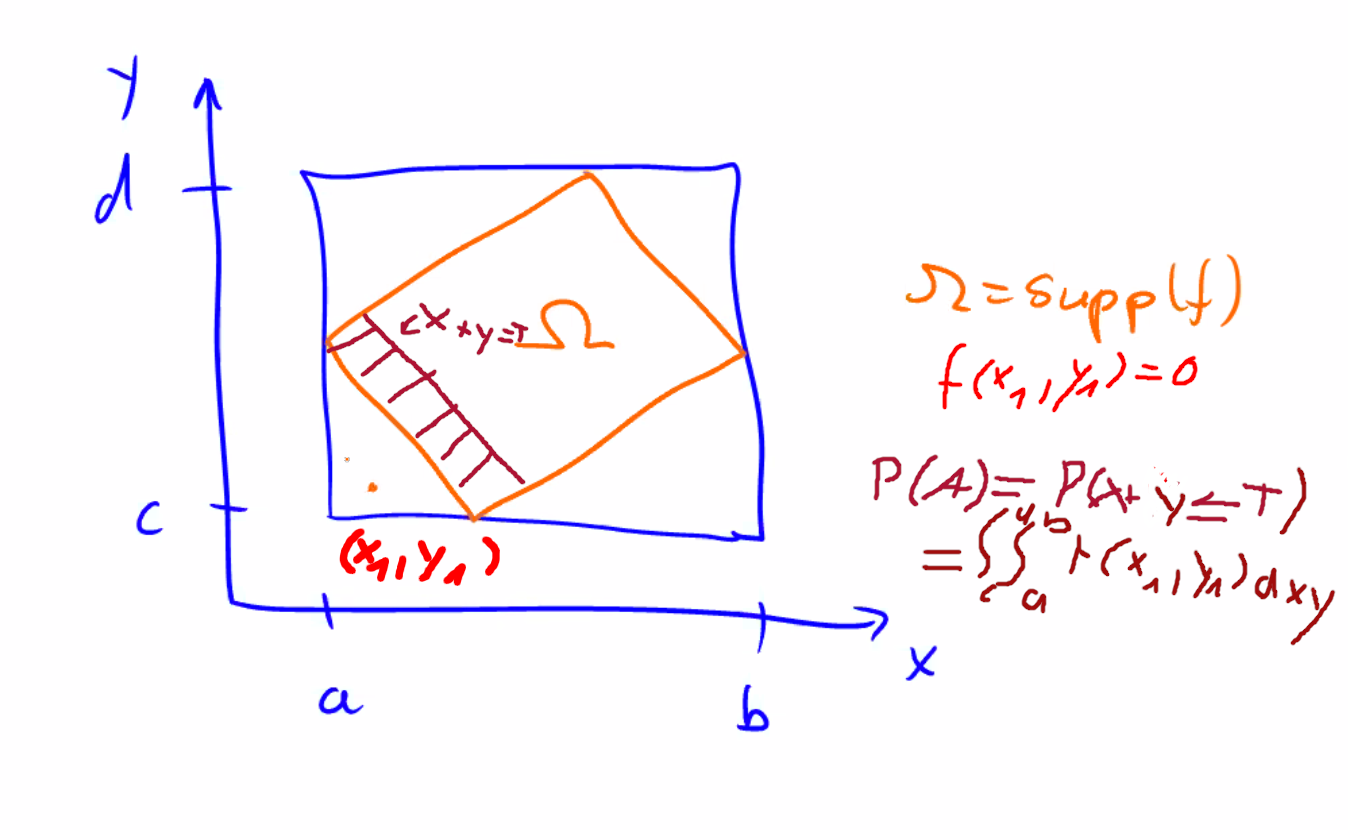
\includegraphics[width=256px]{probsupport.png}\\
	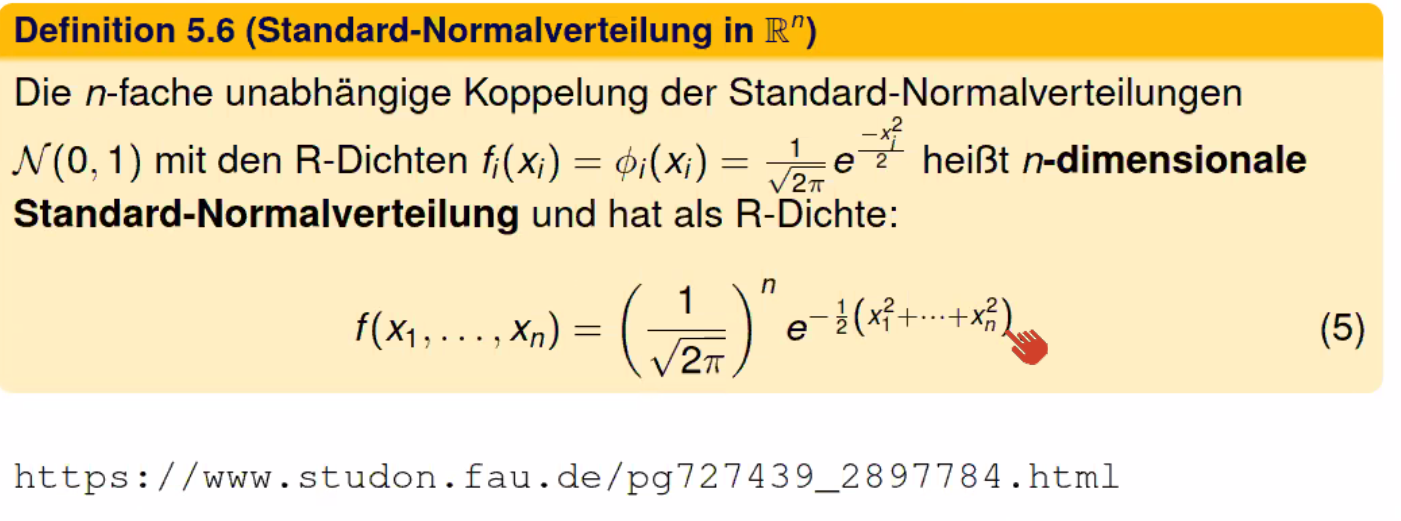
\includegraphics[width=256px]{NormalverteilInN_Dim.png}\\
	\includegraphics[width=256px]{Überblick.png}\\
	\\\\
	Gemeinsame Dichte, die sich aus übergangsdichten zusammensetzt ein W-Maß ist:\\
	$f^{i-1}_i \geq 0$ W-Dichte\\
	$\sum_{\omega_i\in\Omega_i} f^{i-1}_i(\omega_1,\dots, \omega_i)=1$\\
	$f(\omega_1,\dots,\omega_n) = f_1(\omega_1)f_2(\omega_1,\omega_2)\dots\geq 0$\\
	$\sum_{\omega_1\in\Omega_1} \dots \sum_{\omega_n\in\Omega_n}  = 1$ (man zieht ja in jedem schritt ein $\omega_k$ )\\
	\\
	Bei merhfachen Ziehen ohne zurücklegen hat jedes Ergebnis die gleiche Wahrscheinlichkeit\\
	Anzahl permutationen von n aus N Objekten mit Berücksichtigung der Reihenfolge und ohne Wiederholung:\\
	Absteigendes Produkt: $|\Omega_\neq|=N(N-1)(N-2)\dots (N-n+1)= (N)_n$ ist das n-fache absteigende Produkt.\\
	Für N=n ist der Spezialfall $n!$ und $n=0$ liefert N\\
	Daraus folgt auch der Binomialkoeffizient:\\
	von n aus N Objekten ohne Reihenfolge und ohne Wiederholung:\\
	$\binom{N}{k} = \frac{N!}{k!(N-k)!} = \frac{1}{k!}\frac{N!}{(N-k)!} = \frac{(N)_k}{(K)_k}$\\
	Der Twist an der Sache ist, dass man diese Definiton auf Reelle erweitern kann:\\
	$(N)_k = N(N-1)\dots (N-k+1)$ geht genau so, wenn $N\in\mathbb{R}$ und $k\in\mathbb{N} $\\
	Diese definition gilt nicht nur für natürliche Werte, sondern insgesamt für alle $N\in\mathbb{R}$ mit $N<n$\\
	$f(\omega_1,\dots,\omega_n) = \frac{(K)_k (N-K)_{n-k}}{(N)_n}$ mit $k=\sum^n_{i=1} \omega_i$\\
	Daraus folgt $P(B_k) = \binom{n}{k} \frac{(K)_k (N-K)_{n-k}}{(N)_n} = \frac{\binom{K}{k}\binom{N-K}{n-k}}{\binom{N}{n}}$\\
	Ein Beispiel:\\
	Aus 100 Werkstücken sind $N-K=10$ defekt. Mit $\omega_1 = 1$\\
	Das Ereignis $f(0,1,0,1,0) = \frac{10}{100}\frac{90}{99}\frac{9}{98}\frac{89}{97}\frac{8}{96} = \frac{(90)_2 (10)_3}{(100)_5}$\\
	Der Wert ist also nur von der Anzahl, nicht aber von der Reihenfolge der defekten Werkstücke abhängig.\\
	$f(\omega_1,\dots,\omega_n) = \frac{(K)_k (N-K)_{n-k}}{(N)_n}$\\
	Anordnugnsproblem: wir ordnen k aus n Elementen an\\
	Variation: -mit Reihenfolge. $V_{n,k} = \frac{n!}{(n-k)!} = (n)_k$\\
	Kombination: ohne Reihenfolge. $K_{n,k} = \frac{n!}{k!(n-k)!} =\binom{n}{k}$ (es fallen die $k!$ anordnungsvarianten weg)
	\section{Bildmodelle und Zufallsvariable}
	
\end{document}